\documentclass[a4paper,12pt]{report}
\pagestyle{plain}
\usepackage[hidelinks]{hyperref}

\usepackage[fontsize=12pt]{scrextend}

\newcommand{\ud}{\,\mathrm{d}}
\usepackage[utf8]{inputenc}
\usepackage[margin=2cm]{geometry}
\renewcommand{\baselinestretch}{2}
\usepackage{graphicx}
\graphicspath{{../pdf/}{../jpeg/}}
\DeclareGraphicsExtensions{.pdf,.jpeg,.png}
\usepackage{mathtools}
\usepackage{amsmath,amssymb, amsthm, bbm}
\usepackage{epsfig}
\usepackage{varioref}
\usepackage{arydshln}
\usepackage{paralist}
\usepackage{algpseudocode}
\usepackage{algorithm}
\usepackage{algorithmic}
\usepackage{color}
\usepackage{setspace}
\newtheorem{theorem}{Theorem}
\newtheorem{lemma}{Lemma}
\newtheorem{remark}{Remark}
\newtheorem{definition}{Definition}
\newtheorem{proposition}{Proposition}
\newtheorem{conjecture}{Conjecture}
\usepackage{caption}
\usepackage[skip=0cm,list=true,labelfont=it]{subcaption}
\usepackage{subcaption} % For subfigures
\usepackage{adjustbox} % Add this package
\usepackage{graphicx}
\usepackage{cite}
\usepackage{booktabs}
\usepackage{pdfpages}

\usepackage{xcolor, soul, framed}

\usepackage[backend=bibtex]{biblatex}
\addbibresource{Bibliography.bib}
\newcommand{\eng}[1]{\textenglish{#1}}

\usepackage{fancyhdr}
\usepackage[hebrew,english]{babel}
\DeclareUnicodeCharacter{05D0}{\hebalef}
\DeclareUnicodeCharacter{05D1}{\hebbet}
\DeclareUnicodeCharacter{05D2}{\hebgimel}
\DeclareUnicodeCharacter{05D3}{\hebdalet}
\DeclareUnicodeCharacter{05D4}{\hebhe}
\DeclareUnicodeCharacter{05D5}{\hebvav}
\DeclareUnicodeCharacter{05D6}{\hebzayin}
\DeclareUnicodeCharacter{05D7}{\hebhet}
\DeclareUnicodeCharacter{05D8}{\hebtet}
\DeclareUnicodeCharacter{05D9}{\hebyod}
\DeclareUnicodeCharacter{05DA}{\hebfinalkaf}
\DeclareUnicodeCharacter{05DB}{\hebkaf}
\DeclareUnicodeCharacter{05DC}{\heblamed}
\DeclareUnicodeCharacter{05DD}{\hebfinalmem}
\DeclareUnicodeCharacter{05DE}{\hebmem}
\DeclareUnicodeCharacter{05DF}{\hebfinalnun}
\DeclareUnicodeCharacter{05E0}{\hebnun}
\DeclareUnicodeCharacter{05E1}{\hebsamekh}
\DeclareUnicodeCharacter{05E2}{\hebayin}
\DeclareUnicodeCharacter{05E3}{\hebfinalpe}
\DeclareUnicodeCharacter{05E4}{\hebpe}
\DeclareUnicodeCharacter{05E5}{\hebfinaltsadi}
\DeclareUnicodeCharacter{05E6}{\hebtsadi}
\DeclareUnicodeCharacter{05E7}{\hebqof}
\DeclareUnicodeCharacter{05E8}{\hebresh}
\DeclareUnicodeCharacter{05E9}{\hebshin}
\DeclareUnicodeCharacter{05EA}{\hebtav}

\input{myshorts}
\usepackage{amsfonts,amssymb,amsmath,bm,mathtools,stackrel,epsfig,amsthm}
\begin{document}
	\begin{titlepage}
		\begin{center}
			
			
\includegraphics[width=1\textwidth]{Figs/BGU.png}\\
			\huge{\textbf{Mind The Gap - A Discrepancy-Based Computational Analysis of Literary Character Networks}}
			
			\vspace{1cm}
			\large{Submitted in partial fulfillment of the requirements for the Master Degree in the Faculty of Engineering, Ben-Gurion University}
			
			\vspace{1cm}
			
			\Large{Omri Rafaeli\\	
			Supervised by: Dr. Dan Vilenchik, Prof. Itay Marienberg-Milikowsky}
			
		
			
		\end{center}
	\end{titlepage}
%	\maketitle
	\newpage
		\begin{titlepage}
		\begin{center}
			%	\vspace*{1cm}
			
			
\includegraphics[width=1\textwidth]{Figs/BGU.png}\\
			\huge{\textbf{Mind The Gap - A Discrepancy-Based Computational Analysis of Literary Character Networks}}
			
						
			\small{
				Author: Omri Rafaeli ……………… Date: 16.3.26 ………………\\
				Supervisor: Dr. Dan Vilenchik & Prof Itay Marienberg-Milikowsky\\

				Name: ………………………… ………………………… Date: ………
                
				Name: ………………………… ………………………… Date: ………
                
				Chairman of graduate studies committee:\\
				Name: ………………………… ………………………… Date: ………
                			}
			
		\end{center}
	\end{titlepage}

\pagenumbering{roman} % Roman numerals for beginning
\setcounter{page}{2} % Start at 2 so title page isn't numbered

%	\newpage
\selectlanguage{hebrew}
\chapter*{תקציר}ניתוח ספרותי נשען לעיתים קרובות על הבנת מערכות היחסים בין דמויות, משימה שבאופן מסורתי מבוצעת באמצעות ספירות פשוטות של הופעה משותפת בטקסט. עם זאת, מחקר זה מציע גישה חדשה לניתוח הדינמיקה בין דמויות באמצעות שימוש במספר שיטות חישוביות המאפשרות ללכוד מערכות יחסים מורכבות יותר בטקסטים ספרותיים. במחקר נעשה שימוש בטכניקות מתקדמות של עיבוד שפה טבעית ולמידה עמוקה במטרה לחשוף תובנות עמוקות יותר לגבי האינטראקציות בין דמויות.

לצורך מידול מערכות היחסים בין הדמויות נעשה שימוש במספר שיטות, ובהן ניתוח הופעה משותפת, ניתוח הטמעות מילים ושיטות נוספות המבוססות על מודל שפה הקשרי, המספקות נקודות מבט שונות על האינטראקציות בין הדמויות – מספירות תדירות פשוטות ועד ייצוגים סמנטיים מורכבים.

כדי לגשר על הפערים בין גישות המידול השונות מוצעת טכניקה חדשה המבוססת על השוואת גרפים באמצעות קיבוץ משקלי הקשתות לקבוצות. שיטה זו מאפשרת לחשב הבדלים משמעותיים בין ייצוגי זוגות דמויות ולזהות באופן יעיל יותר אי־התאמות בין השיטות השונות.

ממצאי המחקר מדגימים את יעילות השיטות החישוביות בניתוח דמויות ספרותיות ואת יכולתה של השיטה המוצעת לחשוף דינמיקות עדינות ולעיתים נסתרות בטקסט, ובכך לתרום להבנה עשירה ומקיפה יותר של מערכות היחסים בין דמויות ולחקר הנרטיב בכלל.

\selectlanguage{english}
%	\newpage
	\chapter*{Abstract}
	Literary analysis often relies on understanding character relationships, a task traditionally managed through basic co-occurrence counts. However, this research proposes a novel approach to analyzing character dynamics by employing multiple computational methods to capture nuanced relationships in literary texts. Our study leverages advanced techniques in Natural Language Processing (NLP) and deep learning to uncover deeper insights into character interactions.

We utilize several methods to model character relationships, including Co-Occurrence Analysis (COO), Word2Vec Embedding Analysis (W2V), and two innovative BERT-based techniques: BERT Average Character Embedding (BACE) and BERT CLS Vector Analysis (BCLS). Each method provides a distinct perspective on character interactions, from simple frequency counts to complex semantic embeddings.

To bridge the gaps between these various modeling approaches, we introduce a novel technique known as the Clustering-Based Graph Difference (CBGD) Method. This method addresses the challenge of comparing graphs derived from different metrics by employing k-means clustering to normalize and bin edge weights. This enables the calculation of meaningful differences between character pair representations, allowing us to identify and explore discrepancies between methods more effectively.

Our research not only demonstrates the effectiveness of these techniques in analyzing literary characters but also highlights how the CBGD Method can reveal subtle and previously overlooked dynamics within the text. By integrating multiple analytical lenses, this study offers a richer and more comprehensive understanding of character relationships, advancing both computational literary analysis and the broader field of narrative studies.

    \chapter*{Acknowledgements}
   I would like to express my sincere gratitude to my supervisor, Dr. Dan Vilenchik, for supporting my choice of this research topic and for encouraging me to pursue the area I am most passionate about and hope to further specialize in. His guidance, insight, and trust throughout this process have been invaluable.

I am also deeply grateful to my second supervisor, Dr. Itay Marienberg-Milikowsky, for his thoughtful feedback, intellectual generosity, and meaningful contribution to this work. His perspective and guidance significantly enriched the development of this thesis.

Finally, and just as importantly, I would like to thank my wonderful wife, Yaara, for her unwavering support, patience, and understanding throughout this journey. I am profoundly grateful for the time and space she allowed me to dedicate to this project. I know it was not always easy, and I could not have completed this work without her love and encouragement.\\
    
	\newpage
	\tableofcontents
	\newpage
	\listoffigures
	\newpage



\newpage
\chapter*{Abbreviations}
\addcontentsline{toc}{chapter}{Abbreviations}

\begin{table}[h!]
\centering
\renewcommand{\arraystretch}{1.3}
\begin{tabular}{@{}ll@{}}
\toprule
\textbf{Abbreviation} & \textbf{Meaning} \\ 
\midrule
AI & Artificial Intelligence \\
BACE & BERT Average Character Embedding \\
BCLS & BERT CLS (Classification Token) Embedding \\
BERT & Bidirectional Encoder Representations from Transformers \\
CBGD & Clustering-Based Graph Difference \\
CLS & [CLS] token used for sentence-level embeddings in BERT \\
COO & Co-Occurrence (count-based character relationship method) \\
CRELAT & Character Relationships Analyzing Tool (software library developed for this study) \\
DF & Disagreement Factor (multi-graph gap metric) \\
ML & Machine Learning \\
NER & Named Entity Recognition \\
NLP & Natural Language Processing \\
PCA & Principal Component Analysis \\
W2V & Word2Vec (distributional word embedding model) \\
\bottomrule
\end{tabular}
\end{table}
 
\newpage
\addcontentsline{toc}{chapter}{Notation}

\chapter*{Notation}

\begin{table}[h!]
\centering
\renewcommand{\arraystretch}{1.3}
\begin{tabular}{@{}ll@{}}
\toprule
\textbf{Symbol} & \textbf{Meaning} \\ 
\midrule
$T = \{t_1, t_2, \dots, t_m\}$ & Sequence of tokens representing the text. \\
$\mathcal{C} = \{c_1, c_2, \dots, c_k\}$ & Set of character entities in the book. \\
$W_i$ & Sliding window of tokens used for co-occurrence counting. \\
$w$ & Window size (number of tokens per window). \\
$\mathbf{M}$ & Co-occurrence matrix representing pairwise counts of characters. \\
$\mathbf{M}(a,b)$ & Number of windows where characters $c_a$ and $c_b$ co-occur. \\
$\mathbf{v}_a$ & Embedding vector representing character $c_a$. \\
$\text{Sim}(c_a, c_b)$ & Cosine similarity between characters $c_a$ and $c_b$. \\
$P_a = \{p_1, p_2, \dots, p_k\}$ & Set of passages in which character $c_a$ appears. \\
$\mathbf{e}_i$ & BERT contextual embedding of character $c_a$ in passage $p_i$. \\
$\mathbf{v}_a^{\text{CLS}}$ & CLS-based embedding vector for character $c_a$. \\
$G = (V, E)$ & Graph where vertices $V$ are characters and edges $E$ represent relationships. \\
$w_{ab}^{(i)}$ & Edge weight between $a$ and $b$ in graph $G_i$. \\
$C(w_{ab}^{(i)})$ & Cluster assignment of edge weight $w_{ab}^{(i)}$ after $k$-means clustering. \\
$k$ & Number of clusters used for weight binning. \\
$w_{ab}^{\Delta}$ & Difference in cluster numbers between two graphs (gap weight). \\
$DF_{ab}$ & Disagreement Factor across multiple graphs for edge $(a,b)$. \\
$G_{\Delta}$ & Difference graph representing discrepancies between two graphs. \\
\bottomrule
\end{tabular}
\end{table}
	
%%%%%%%%%%%%%%%%%%%%%%%%%%%%%%%%%%%%%%%%%%%%%%%%%%%%%%%%	
	\newpage	
 
\pagenumbering{arabic} % arabic numbering for main part
\chapter{Introduction}
\label{sec:intro}
Understanding character relationships in literature is a complex and multifaceted task that has traditionally relied on various methodologies such as co-occurrence counts, direct quotations, and manual annotation. Traditional methods, such as counting the frequency of co-occurrence or analyzing dialogue exchanges, provide foundational insights into character dynamics. This computational turn in literary studies builds on earlier quantitative approaches in digital humanities, most notably the work of Moretti and collaborators, who advocated for distant reading and formalized literary structures at scale \cite{MORETTI2011Quantitative}.However, these approaches often offer a limited view, constrained by their simplicity and the static nature of their analysis.

In recent years, Natural Language Processing (NLP) systems have achieved remarkable success in automating a wide range of administrative and informational language tasks — activities that humans perform through structured and rule-based thinking, such as summarization, categorization, or entity extraction. Yet, when these computational tools are applied to literary texts, they encounter a very different challenge. Literature operates not through explicit logic but through ambiguity, emotional resonance, and narrative nuance. As a result, standard NLP techniques, while powerful for well-defined linguistic tasks, often produce flattened representations of literary phenomena — capturing structure but missing texture.

This tension forms the core of our research question:
Can computational models, originally designed for surface-level text understanding, be repurposed to uncover subtle aspects of literary meaning that might otherwise escape the human eye?

Rather than asking NLP models to “understand” literature in a human sense, we explore how their differences — the gaps between distinct computational representations — might themselves become sources of insight. Each model offers a unique way of perceiving the text: co-occurrence networks focus on proximity, Word2Vec captures distributional similarity, and BERT-based embeddings represent deeper contextual semantics. The disagreements among these models are not mere errors; they reveal fractures in representation that reflect the underlying richness of the literary work itself.

Our hypothesis is that within these discrepancies lie patterns of meaning — latent dynamics, tensions, or associations between characters — that are intuitively sensed by human readers but remain elusive to formal analysis. By treating the inconsistencies among NLP models as data rather than noise, we seek to transform computational limitations into interpretive opportunities.

To investigate this, we implemented and compared several methods for modeling character relationships:

\begin{itemize}
\item \textbf{Classical Methods:}
\begin{itemize}
\item \textbf{Co-Occurrence (COO):} Counts the frequency with which pairs of characters appear together within a defined textual window \cite{LABATUT}. See \ref{COO}.
\item \textbf{Word2Vec (W2V):} Captures character relationships through semantic embeddings derived from surrounding contexts. \cite{WORD2VEC} See \ref{W2V}.
\end{itemize}
\item \textbf{Advanced Methods:}
\begin{itemize}
\item \textbf{BERT Average Character Embedding (BACE):} Extracts contextual embeddings from passages where characters appear, using BERT \cite{BERT} to capture nuanced contextual meaning. See \ref{BACE}.
\item \textbf{BERT CLS Embedding (BCLS):} Represents each passage using BERT’s global CLS token \cite{BERT}, emphasizing overall narrative context. See \ref{BCLS}.
\end{itemize}
\end{itemize}

Despite their sophistication, these approaches differ not only in technique but in the type of relationship they encode. The resulting “gap” between models — between what each method sees and what it overlooks — is central to this study.
We propose that by systematically identifying and analyzing these gaps, one can expose hidden layers of meaning in literary texts. This idea led us to develop the Clustering-Based Graph Difference (CBGD) method, designed specifically to quantify and interpret discrepancies between character-relationship graphs derived from multiple modeling lenses. Instead of viewing variation as a flaw, CBGD turns it into a measurable phenomenon — a way to map the “interpretive space” that different algorithms carve out within the same text.

In essence, this research seeks to bridge the divide between computational precision and literary interpretation. It asks whether the friction between models — the points where their outputs diverge — can serve as a lens for understanding aspects of narrative complexity that defy straightforward modeling.
By doing so, we propose a new way of engaging with AI in the humanities: not as a replacement for human reading, but as a mirror that reveals the multidimensional nature of textual meaning — a mirror built from algorithms that see differently.

\section{Thesis Layout}
The remainder of this thesis is organized as follows:

\begin{itemize}
    \item \textbf{Chapter 1 – Introduction:} Presents the motivation and research question that guide this work. It discusses the challenges of applying computational models to literary texts and introduces the idea of using discrepancies between NLP models as interpretive signals rather than errors. The chapter concludes with a description of the main conceptual and technical contributions of the research.
    
    \item \textbf{Chapter 2 – Machine Learning:} Provides an overview of the core principles of machine learning, including supervised and unsupervised learning paradigms, representation learning, and their relevance to computational text analysis. This chapter establishes the theoretical basis for the modeling approaches used later in the thesis.
    
    \item \textbf{Chapter 3 – Natural Language Processing:} Introduces the foundations of NLP as a discipline that enables machines to process, represent, and generate human language. It reviews traditional and modern approaches, levels of linguistic analysis, key applications, and the challenges that arise when modeling natural language computationally.
    
    \item \textbf{Chapter 4 – Methodology:} Describes the methodological framework developed for this study. It details the preprocessing pipeline, character relationship modeling methods (COO, W2V, BACE, BCLS), and the novel Clustering-Based Graph Difference (CBGD) method used to quantify discrepancies between different network representations. The chapter also introduces the CRELAT software library, which implements the full analysis pipeline.
    
    \item \textbf{Chapter 5 – Evaluation:} Explains the evaluation process of the proposed methods. It combines quantitative analyses—such as model correlation, sensitivity testing, and consistency measures—with qualitative, reader-oriented assessments designed to test the interpretive potential of the gap networks.
    
    \item \textbf{Chapter 6 – Results:} Summarizes the key empirical findings from the analyses, including observed correlations, model divergences, and interpretive “hot spots” revealed by the CBGD method. It discusses the implications of these findings for both computational and literary analysis.
    
    \item \textbf{Chapter 7 – Conclusion:} Concludes the thesis by summarizing the main insights, discussing methodological and interpretive limitations, and suggesting directions for future work—such as cross-book comparison, large-scale corpus analysis, and integration with other computational models of narrative.
\end{itemize}

Each chapter builds upon the previous one, moving from theoretical foundations to practical implementation and interpretive evaluation. Together, they establish a comprehensive framework for exploring how computational differences can enrich the study of literature.
\section{Research Contribution and Implementation}
This thesis contributes both conceptually and technically to the study of computational literary networks.

On the conceptual level, it introduces a novel methodological framework for analyzing discrepancies between multiple Natural Language Processing (NLP) models of character relationships. The proposed method, termed the \textbf{Clustering-Based Graph Difference (CBGD)}, enables systematic quantification of the “gaps” between graphs generated by heterogeneous modeling approaches such as Co-Occurrence (COO), Word2Vec (W2V), and BERT-based embeddings (BACE and BCLS). By reframing disagreement between models as meaningful data rather than noise, this framework establishes a new way to interpret the computational modeling of literature.

On the technical level, this thesis presents the design and development of an open-source Python library named \textbf{CRELAT (Character Relationships Analyzing Tool)}. 
CRELAT automates the full research pipeline—from text preprocessing and character alias consolidation to network generation, graph comparison, and visualization of discrepancies. 
The library not only operationalizes the CBGD methodology but also provides a general-purpose infrastructure that allows researchers to apply, extend, and visualize character relationship analyses across different literary corpora.

The CRELAT library is freely available as open source at:
\href{https://github.com/omrir7/CRELAT.git}{\texttt{https://github.com/omrir7/CRELAT.git}}

Together, these contributions bridge the gap between computational precision and humanistic interpretation, offering both a conceptual framework and a practical tool for exploring how algorithms can highlight the multidimensional nature of literary meaning.
%%%%%%%%%%%%%%%%%%%%%%%%%%%%%%%%%%%%%%%%%%%%%%%%%%%%%%%%%%%%%%%%%%%%%%%%%%%%%%%%%%%%%%%%%%%%%%%%%%%
\chapter{Machine Learning}
\label{chap:ML}

Machine Learning (ML) provides the computational foundation for most modern Natural Language Processing (NLP) techniques employed in this study. 
At its core, ML refers to a set of algorithms and models that learn patterns from data rather than relying on explicit, rule-based programming. \cite{MITCHELL1997}
In literary text analysis, ML enables systems to generalize from examples—such as word contexts or syntactic patterns—and to represent linguistic or semantic relationships in a multidimensional mathematical space. 

\section{Supervised and Unsupervised Learning}
Machine learning paradigms are generally divided into two main categories: \textbf{supervised} and \textbf{unsupervised} learning. 
In supervised learning, a model is trained on labeled data, where each input example has a corresponding target output. \cite{VAPNIK1995}
The goal is to minimize the difference between the predicted and true outputs, using metrics such as cross-entropy or mean-squared error. \cite{HASTIE2009}
Examples include text classification and sentiment analysis.

Unsupervised learning, by contrast, operates without labeled outputs. 
It aims to uncover hidden structure in the data by identifying clusters, distributions, or lower-dimensional representations. 
For example, clustering algorithms like $k$-means group similar observations, while dimensionality-reduction methods such as PCA (Principal Component Analysis) project data into a space that preserves meaningful variance. 
The methods used in this thesis—Word2Vec, BERT-based embeddings, and clustering of graph weights—are all grounded in the principles of unsupervised learning. 
They learn from the co-occurrence structure of words and names in the text, identifying implicit patterns that are not manually annotated.\cite{MURPHY2012}

\section{Representation Learning}
A central concept in modern ML is \textbf{representation learning}—the ability of a model to transform raw data into a numerical representation that captures salient features of the underlying phenomenon. 
Modern embedding approaches rely on distributional and geometric principles of representation learning \cite{TURNEY2010}, where semantic relationships are encoded as spatial proximity in high-dimensional vector spaces \cite{HAMILTON2016Embeddings}.
In text modeling, this is typically achieved by mapping each token, sentence, or document into a vector space, where geometric relationships correspond to semantic similarity. 
This principle is evident in the Word2Vec model, where proximity in the embedding space reflects contextual similarity, and in deep contextual models such as BERT, where token embeddings are dynamically adjusted based on their surrounding words. 

Representation learning provides the theoretical bridge between the mathematical world of vectors and the interpretive world of literary meaning. 
By encoding characters, words, and scenes as vectors, it becomes possible to model abstract relationships—such as thematic resonance or narrative proximity—through geometric operations. \cite{BISHOP2006}
This allows us to study the “shape” of literary relationships using tools borrowed from data science.
\chapter{Natural Language Processing}
\label{chap:NLP}

Natural Language Processing (NLP) is a subfield of artificial intelligence and linguistics that focuses on the interaction between computers and human language. \cite{JURAFSKY}
Its goal is to enable machines to read, interpret, and generate human language in a way that is both meaningful and useful. 
NLP combines methods from computer science, linguistics, and statistics to analyze large amounts of textual data and to uncover patterns that would otherwise be inaccessible to manual analysis.

\section{Language as Data}
Human language is inherently ambiguous, context-dependent, and full of subtle cues such as tone, irony, and metaphor. 
From a computational point of view, language can be represented as sequences of symbols—words, phrases, or sentences—that carry information. 
The central challenge of NLP is to convert these symbolic structures into numerical representations that algorithms can process while still preserving their linguistic and semantic richness. 
This transformation allows computers to perform a variety of language-based tasks such as classification, translation, or summarization.

\section{Levels of Linguistic Analysis}
NLP operates on several levels of linguistic structure:

\begin{itemize}
    \item \textbf{Morphological level:} the study of word formation, including prefixes, suffixes, and stems. For example, identifying that "running" and "ran" share the same root "run."
    \item \textbf{Syntactic level:} the analysis of grammatical relationships between words within a sentence, often represented through parsing trees.
    \item \textbf{Semantic level:} the extraction of meaning from text, such as understanding that "cat" and "dog" are both animals but distinct entities.
    \item \textbf{Pragmatic level:} understanding meaning in context, such as interpreting irony or recognizing implied intent.
\end{itemize}

Each of these layers contributes to building a computational understanding of how words combine to create meaning.

\section{Traditional and Modern Approaches}
Historically, NLP relied heavily on rule-based systems that encoded linguistic knowledge manually. 
Early systems used handcrafted grammars and lexicons \cite{MANNING1999}, which worked well for limited, structured domains but were difficult to scale. 
With the rise of machine learning, especially statistical and neural models, NLP shifted toward data-driven approaches. 
Instead of relying on explicit linguistic rules, models began to learn from large corpora of text, identifying patterns of usage automatically.

This shift gave rise to techniques such as \textbf{n-gram models}, which estimate the probability of word sequences \cite{BROWN1992}; and later to \textbf{embedding models}, which represent words as dense vectors in high-dimensional space. 
Modern NLP, powered by deep learning architectures \cite{LECUN2015} such as recurrent neural networks (RNNs) \cite{RUMELHART1986} \cite{HOCHREITER1997}, convolutional neural networks (CNNs), and especially transformers, has achieved remarkable progress in understanding context \cite{GOODFELLOW2016}, disambiguating meaning, and generating coherent text.
The introduction of the transformer architecture \cite{VASWANI2017Attention} marked a fundamental shift toward attention-based contextual modeling, enabling large-scale pretraining strategies such as BERT.

\section{Text Representation}
One of the fundamental principles in NLP is that linguistic meaning can be represented geometrically. 
Words, sentences, and documents can be mapped into numerical vectors where distance and direction encode relationships such as similarity or analogy. \cite{CHURCH1990}
For example, the relationship between “king” and “queen” can be expressed as a consistent vector offset similar to that between “man” and “woman.”  

These vector representations—known as \textbf{embeddings}—enable algorithms to perform mathematical operations on language. \cite{BENGIO2003} 
They form the foundation of many downstream NLP tasks, including sentiment analysis, machine translation, and question answering.

\section{Applications}
NLP is now widely used in both research and industry. 
Common applications include:

\begin{itemize}
    \item \textbf{Machine translation:} automatically converting text between languages (e.g., Google Translate).
    \item \textbf{Information retrieval:} finding relevant documents or passages in large corpora.
    \item \textbf{Sentiment analysis:} detecting emotional tone in reviews, social media, or news.
    \item \textbf{Named Entity Recognition (NER):} identifying people, organizations, and locations in text.
    \item \textbf{Summarization and question answering:} generating concise summaries or extracting key information from documents.
\end{itemize}

The success of these applications has been driven largely by the availability of large-scale data and powerful neural architectures such as BERT and GPT, which can capture complex contextual dependencies across entire texts.

\section{Challenges in NLP}
Despite its success, NLP still faces several open challenges. 
Ambiguity, figurative language, and cultural context remain difficult to model computationally. 
Models often struggle to capture nuances such as sarcasm, metaphor, and emotion—features that are central to human communication. 
Moreover, large language models, while powerful, can reproduce biases present in their training data or fail to provide transparent reasoning. 
As such, interpretability, fairness, and domain adaptation continue to be active research areas.
\chapter{Methodology}
Building on the conceptual framework outlined in the introduction, this chapter presents the methodological foundation of our study. As discussed earlier, our central question concerns whether discrepancies between computational models—each capturing character relationships through a different semantic lens—can serve as meaningful interpretive triggers for literary reading. To explore this, we designed a multi-stage methodology that combines several Natural Language Processing (NLP) techniques for modeling character relationships, followed by a novel computational procedure for identifying and quantifying the gaps between them.
The goal of this chapter is therefore twofold: first, to detail how we construct character relationship networks using both classical and deep-learning-based models; and second, to describe the Clustering-Based Graph Difference (CBGD) method, which allows us to systematically compare these networks and interpret their discrepancies as potential sites of literary insigh
\section{Pre-Processing Pipeline}
\label{pre-process}
\subsection{Data Preprocessing}

The preprocessing phase is essential for transforming the raw book text into a structured format that can be analyzed. The input to the preprocessing pipeline consists of two components: the raw book text and an \texttt{entities} object, which is a 2D array where each row represents a character entity, and each element within the row is a different reference or alias for that character.

The following steps are performed during preprocessing:

\begin{enumerate}
    \item \textbf{Punctuation Removal:} The raw book text is first processed to remove all punctuation marks. This step eliminates unnecessary symbols that do not contribute to the meaning of the text, thereby improving the quality of the data.

    \item \textbf{Stopword Removal:} Next, stopwords are removed from the text. These are common words (such as "the," "is," and "and") that carry little to no semantic meaning. Removing stopwords allows us to focus on the core content and meaning of the text.

    \item \textbf{Entity Referencing Consolidation:} Using the \texttt{entities} object, we consolidate multiple references to the same character into a single, unified name. Each row in the \texttt{entities} array contains all possible aliases or references to a character, and these are mapped to a single name for consistency in the analysis. This ensures that all mentions of a character, regardless of variation, are correctly attributed to the same entity.
\end{enumerate}

Initially, we utilized the Named Entity Recognition (NER) model provided by BOOKNLP, a computational framework for large-scale narrative analysis \cite{BAMMAN}. However, we found that the NER model was not sufficiently robust for our needs. Consequently, we decided not to focus heavily on the NER component and opted to use the \texttt{entities} object as input to streamline the preprocessing process and maintain a focus on the core analysis.


\section{Characters Relationship Modeling Methods}
\subsection{COO - Co-Occurrences Counting}
\label{COO}
The Co-Occurrences (COO) method is a classical approach for character relationship modeling based on counting the frequency with which characters appear together in the text. This method relies on a sliding window of a predetermined length, which moves sequentially over the text. For each pair of characters that appear within the window, a co-occurrence count is incremented. 

Formally, let the text be represented as a sequence of tokens $T = \{t_1, t_2, \dots, t_m\}$, where each token corresponds to a word or punctuation mark in the text. Let $\mathcal{C} = \{c_1, c_2, \dots, c_k\}$ be the set of characters in the text. We define a sliding window of size $w$, such that for any window $W_i = \{t_i, t_{i+1}, \dots, t_{i+w-1}\}$, the co-occurrence of two characters $c_a$ and $c_b$ is incremented if both $c_a$ and $c_b$ are mentioned within the window.

The co-occurrence matrix $\mathbf{M}$ is then defined as:

\[
\mathbf{M}(a, b) = \sum_{i=1}^{m-w+1} \mathbb{I}(c_a \in W_i \land c_b \in W_i)
\]

where $\mathbb{I}(\cdot)$ is the indicator function that returns 1 if the condition is true and 0 otherwise. Each entry $\mathbf{M}(a, b)$ represents the number of times characters $a$ and $b$ co-occurred within the sliding window. This matrix provides a direct representation of the strength of relationships between characters based purely on their proximity in the text. 

The COO method captures interactions that may be implicit, such as characters appearing in the same scene or being mentioned together in a narrative, without necessarily engaging in direct dialogue. This method serves as a fundamental approach to relationship modeling in character networks, offering insights into the frequency of character pairings throughout the text.

\subsection{W2V - Word2Vec}
\label{W2V}
The Word2Vec (W2V) method models character relationships based on semantic similarity, using word embeddings to represent each character within the book. In this approach, we fine-tune a pre-trained Word2Vec model on the specific text of the book, allowing the model to adjust its word embeddings to the particular context and vocabulary of the narrative.

The process begins with fine-tuning the Word2Vec model on the book text, which consists of a set of tokens $T = \{t_1, t_2, \dots, t_m\}$. Word2Vec learns a dense vector representation for each token such that words appearing in similar contexts are closer in the embedding space \cite{MIKOLOV2013}. After fine-tuning, each character $c_a \in \mathcal{C}$ is associated with an embedding vector $\mathbf{v}_a \in \mathbb{R}^d$, where $d$ is the dimensionality of the embedding space.

Once embeddings for all characters are obtained, we define the relationship between two characters $c_a$ and $c_b$ as the cosine similarity \cite{MIKOLOV2013Distributed} between their embedding vectors:

\[
\text{Sim}(c_a, c_b) = \frac{\mathbf{v}_a \cdot \mathbf{v}_b}{\|\mathbf{v}_a\| \|\mathbf{v}_b\|}
\]

Here, $\mathbf{v}_a \cdot \mathbf{v}_b$ denotes the dot product between the two vectors, and $\|\mathbf{v}_a\|$ and $\|\mathbf{v}_b\|$ are the Euclidean norms of the vectors. The resulting cosine similarity ranges from $-1$ to $1$, where a value of $1$ indicates identical embeddings, $0$ indicates orthogonal (unrelated) embeddings, and $-1$ indicates diametrically opposed embeddings.

This similarity score provides a measure of the semantic relatedness between two characters based on their contextual representation in the book. Characters who frequently appear in similar contexts or share similar roles within the narrative will have higher cosine similarity scores, reflecting stronger relationships in the character network.

The W2V method captures deeper, latent relationships between characters, relying not just on proximity in the text but on the broader context in which their names appear. By leveraging the power of word embeddings, this method can identify nuanced connections between characters that may not be immediately apparent through simple co-occurrence.

\subsection{BACE - BERT Average Character Embedding}
\label{BACE}

The BERT Average Character Embedding (BACE) method leverages the power of contextual embeddings generated by the BERT model to represent the relationships between characters. Unlike traditional methods based on co-occurrence or word2vec, BACE focuses on capturing the rich context in which characters appear within the text \cite{ROGERS2020}.

The process begins by identifying passages where a particular character appears in the book. Once identified, the character's name is masked in the passage, ensuring that the BERT model does not rely solely on the specific name token, but instead generates contextual embeddings based on the surrounding text. Let $P_a = \{p_1, p_2, \dots, p_k\}$ represent the set of passages where character $c_a$ appears.

Each passage $p_i$ containing character $c_a$ is processed by the BERT model, which outputs a sequence of contextual embeddings for each token. The embeddings corresponding to the masked character's position are extracted and denoted as $\mathbf{e}_i$. The final embedding for character $c_a$, denoted as $\mathbf{v}_a$, is obtained by averaging these contextual embeddings over all passages:

\[
\mathbf{v}_a = \frac{1}{k} \sum_{i=1}^{k} \mathbf{e}_i
\]

Here, $k$ is the number of passages in which the character appears, and $\mathbf{e}_i$ represents the contextual embedding for character $c_a$ in passage $p_i$. This averaging process smooths out variations in individual contexts, creating a more stable representation of the character's role in the narrative.

To quantify the relationship between two characters $c_a$ and $c_b$, we calculate the cosine similarity between their respective averaged embeddings.

Higher cosine similarity indicates that the characters appear in similar narrative contexts or have related roles within the story.

The BACE method excels at capturing deep semantic relationships by incorporating the surrounding context of each character's appearances, making it particularly suited for modeling nuanced character interactions that depend on the broader narrative structure.

\subsection{BCLS - BERT CLS Embedding}
\label{BCLS}
The BERT CLS Embedding (BCLS) method offers an alternative approach to capturing character relationships by utilizing the special CLS (classification) token embedding generated by BERT, which represents the entire input sequence. Instead of focusing on the specific contextual embeddings of masked character names, the BCLS method leverages the global representation of the passage provided by the CLS token.

In this method, for each character $c_a$, we gather all the passages $P_a = \{p_1, p_2, \dots, p_k\}$ in which the character appears. Each passage $p_i$ is passed through the BERT model, which produces the CLS token embedding $\mathbf{cls}_i$ for the entire passage. This CLS embedding captures the broader contextual meaning of the sentence or passage as a whole, rather than focusing on the individual tokens. 

The final embedding for the character $c_a$, denoted as $\mathbf{v}_a^{\text{CLS}}$, is then computed by averaging the CLS embeddings across all passages:

\[
\mathbf{v}_a^{\text{CLS}} = \frac{1}{k} \sum_{i=1}^{k} \mathbf{cls}_i
\]

Here, $\mathbf{cls}_i$ represents the CLS token embedding for passage $p_i$, and $k$ is the number of passages where character $c_a$ appears. This averaging process aggregates the global contextual information for the character, providing a holistic representation based on their overall presence in the text.

To determine the relationship between two characters $c_a$ and $c_b$, we calculate the cosine similarity.
The BCLS method excels at capturing global, contextual relationships by considering the entire passage in which characters appear, making it useful for modeling interactions that are more reliant on overarching narrative patterns rather than localized context alone.
Recent work has also explored learning character-level representations directly from novels, evaluating their semantic consistency and narrative grounding \cite{INOUE2022Learning}. Our approach differs in that we explicitly compare heterogeneous modeling lenses rather than optimizing a single representation.

\section{Cluster-Based Graph Difference (CBGD) Method}
\label{CBGD}
Character relationship modeling naturally lends itself to graph-theoretic formalization, where vertices represent entities and weighted edges encode relational strength \cite{NEWMAN2010Networks}.
The goal of the Cluster-Based Graph Difference (CBGD) method is to quantify the gaps between two graphs, \( G_1 \) and \( G_2 \), which represent relationships between characters across different semantic lenses. Each edge in the graphs is weighted by a metric corresponding to the relationship strength between two characters, such as co-appearance counts or cosine similarity derived from Word2Vec. The challenge lies in defining a meaningful graph difference operation, as there is no standard method for subtracting graphs like there is for real numbers. Graph comparison remains an open methodological challenge, with numerous distance measures proposed for dynamic and weighted networks \cite{DONNAT2018GraphComparison}. Our approach differs by discretizing heterogeneous edge weights prior to comparison.


\subsection{Notation}

Let \( G_1 = (V_1, E_1) \) and \( G_2 = (V_2, E_2) \) be two graphs with vertex sets \( V_1 \) and \( V_2 \), and edge sets \( E_1 \) and \( E_2 \), respectively. The vertices \( V \) represent characters, and the edges \( e_{ab} \) represent the relationships between characters \( a \) and \( b \). The weight of an edge in graph \( G_1 \) is denoted by \( w_{ab}^{(1)} \), while the weight of the corresponding edge in graph \( G_2 \) is denoted by \( w_{ab}^{(2)} \).

\subsection{Naive Difference Approach}

A naive approach to computing the graph difference is to calculate the absolute difference between the edge weights for each pair of characters. Let \( |E_1| = |E_2| \), then for each edge \( e_{ab} \), the difference is computed as:

\begin{equation}
    \Delta w_{ab} = | w_{ab}^{(1)} - w_{ab}^{(2)} |
\end{equation}

However, this method has a major drawback when the metrics used to define the weights \( w_{ab}^{(1)} \) and \( w_{ab}^{(2)} \) differ in scale. For example, co-appearance counts can range in the hundreds, while cosine similarity values are bounded between \([-1, 1]\). The units do not match, making the absolute difference ineffective.

\subsection{Normalization and Clustering}

To address this issue, we first normalize the edge weights by applying a binning strategy based on clustering. Specifically, we use the \( k \)-means clustering algorithm to categorize the edge weights into discrete bins, which allows for a more interpretable difference measure.

Let the set of edge weights in \( G_1 \) be denoted by \( \{w_{ab}^{(1)}\}_{e_{ab} \in E_1} \), and similarly for \( G_2 \). We cluster the edge weights into \( k \) clusters using \( k \)-means, where each cluster represents a range of weights. Define the clustering function as:

\begin{equation}
    C(w_{ab}^{(i)}) = c_{ab}^{(i)}, \quad i = 1, 2
\end{equation}

where \( C(w_{ab}^{(i)}) \) assigns the weight \( w_{ab}^{(i)} \) to cluster \( c_{ab}^{(i)} \), and \( c_{ab}^{(i)} \in \{1, \dots, k\} \).

\subsection{Choosing \( k \)}
\subsubsection{Choosing $k$}
\label{sec:choosing_k}

The value of $k$, the number of clusters used for weight binning, is a critical hyperparameter in the \textsl{k}-means clustering process. An appropriate selection of $k$ is essential to ensure that the character relationship strengths (edge weights) are grouped into meaningful, distinct clusters for the subsequent calculation of discrepancies.

We determine the optimal $k$ for the set of edge weights $\left\{w_{ab}^{(i)}\right\}_{e_{ab} \in E_{i}}$ by employing the \textbf{Elbow Method}. This heuristic involves running the \textsl{k}-means clustering algorithm for a range of potential values of $k$ and calculating the \textbf{Within-Cluster Sum of Squares (WCSS)}, also known as Inertia, for each resulting partition. The WCSS measures the compactness of the clustering by summing the squared Euclidean distances between each data point and the centroid of its assigned cluster:

\begin{equation}
\text{WCSS}_{k} = \sum_{j=1}^{k} \sum_{w \in C_{j}} \left\|w - \mu_{j}\right\|^2
\end{equation}

where $C_{j}$ is the $j$-th cluster and $\mu_{j}$ is its centroid.

The WCSS is then plotted against $k$. As $k$ increases, the WCSS naturally decreases. The optimal value for $k$ is located at the ``elbow'' point of this curve, where the marginal gain from adding an extra cluster (the decrease in WCSS) sharply diminishes. This point represents the best trade-off between clustering resolution and minimizing the loss of information.

While the selection is inherently heuristic, we choose $k$ based on minimizing the relative rate of decrease in WCSS, effectively locating the knee of the curve:
\begin{equation}
k = \underset{k}{\operatorname{argmin}} \left( \frac{\text{WCSS}_{k} - \text{WCSS}_{k+1}}{\text{WCSS}_{k-1} - \text{WCSS}_{k}} \right) 
\end{equation}



The selected value of $k$ is then used to discretize the continuous edge weights $w_{ab}^{(i)}$ into cluster assignments $c_{ab}^{(i)} \in \{1, \dots, k\}$, which are directly comparable across different modeling lenses.
\
\subsection{Graph Difference Computation}

Once the clusters are assigned, we compute the graph difference, denoted as \( G_{\Delta} = (V, E_{\Delta}) \), where \( V = V_1 = V_2 \). The weight of each edge in the difference graph is defined as the absolute difference in cluster assignments:
\begin{equation}
    w_{ab}^{\Delta} = | c_{ab}^{(1)} - c_{ab}^{(2)} |
\end{equation}

The resulting graph \( G_{\Delta} \) quantifies the gaps between the two input graphs \( G_1 \) and \( G_2 \) in terms of the difference in their cluster assignments. Lower values of \( w_{ab}^{\Delta} \) indicate that the relationships between characters \( a \) and \( b \) are similarly weighted across the two semantic lenses, while higher values suggest greater disparities.

\subsection{Disagreement Factor for Multiple Graphs}

For scenarios involving more than two graphs, we extend the CBGD method by introducing the Disagreement Factor. Let $\mathcal{G} = \{G_1, G_2, \dots, G_n\}$ represent the set of $n$ graphs. Each graph $G_i$ has edges weighted by cluster numbers after applying k-means clustering to the original edge weights. Let $c_{ab}^{(i)}$ represent the cluster number assigned to the edge between characters $a$ and $b$ in graph $G_i$.

The Disagreement Factor, $DF_{ab}$, for the pair $(a,b)$ is then defined as the sum of absolute differences between cluster numbers across all graph pairs:

\[
DF_{ab} = \sum_{i=1}^{n-1} \sum_{j=i+1}^{n} |c_{ab}^{(i)} - c_{ab}^{(j)}|
\]

This formulation provides a measure of the overall disagreement in the relationship between characters across different representations, based on the differences in cluster assignments. High values of $DF_{ab}$ indicate significant divergence in the character relationship across multiple semantic lenses.



\section{CRELAT - Characters Relationships Analyzing Tool}

The CRELAT (Character Relationships Analyzing Tool) library is designed to facilitate in-depth analysis of character interactions within literary texts. It automates the extraction and visualization of character relationships, providing comprehensive insights into character dynamics across single or multiple books.

\subsection{Preprocessing Pipeline}
CRELAT automates the entire preprocessing pipeline for character relationship analysis as described in \ref{pre-process}.

\subsection{Modeling and Graph Generation}
CRELAT supports four different models for character relationship analysis:
\begin{itemize}
    \item \textbf{COO:} Uses co-occurrence frequency to model relationships by counting how often characters appear together in the same passages or scenes. See Section \ref{COO}.
    \item \textbf{W2V:} Utilizes Word2Vec embeddings to measure character relationship strength based on similarity in contextual words. See Section \ref{W2V}.
    \item \textbf{BACE:} A second BERT-based method that averages the embeddings across all tokens in the character's dialogue. See Section \ref{BACE}.
    \item \textbf{BCLS:} A BERT-based method that calculates relationship strength using the average CLS token from pre-trained BERT models. See Section \ref{BCLS}.

\end{itemize}

For each of these models, CRELAT generates weighted graphs where the vertices represent characters and edges are weighted by the strength of their relationships as computed by the model. These graphs are visualizable and provide insights into the structure of relationships within the text.

\subsection{CBGS Method Integration}
\label{CBGS}
CRELAT incorporates the Clustering-Based Graph Subtraction (CBGS) method for analyzing gaps between character relationship graphs. See section \ref{CBGD}.

\subsection{Cross-Book Analysis}
An advanced feature of CRELAT is the cross-book analysis, which allows users to compare character relationships across multiple texts. By running the relationship models on different books, CRELAT can generate graphs that link characters across different literary works. This feature is particularly useful for studying character archetypes or exploring thematic connections between texts.

\subsection{Visualization and Reporting}
CRELAT provides a comprehensive visualization of character relationship networks using interactive graph visualization tools. Users can explore the centrality, influence, and connections between characters, and the graphs can be exported for further use. Additionally, sentiment analysis is incorporated to evaluate the emotional tone of interactions, providing deeper insights into the narrative structure. Reports, graphs, and character profiles can be exported for sharing or integration into further literary studies.
\chapter{Evaluation}
\label{chap:evaluation}

This chapter details the comprehensive strategy employed to evaluate the computational models and the novel methodology developed in Chapter 4. The evaluation is structured to fulfill two primary goals:
\begin{enumerate}[(i)]
    \item To assess the \textbf{computational validity and robustness} of the underlying network representations (COO, W2V, BACE, BCLS) and the integrity of the \textbf{Clustering-Based Graph Difference (CBGD)} method, ensuring the reliability of discrepancy quantification. This includes the in-depth application of the method to the works of \textbf{Amos Oz}, whose novels, characterized by intricate character interactions, serve as the primary case study for the close analysis of our method.
    \item To rigorously examine the \textbf{interpretive utility} of the generated "gaps," specifically verifying whether the discrepancies between computational models function as effective and non-trivial triggers for humanistic close reading, consistent with the reader-oriented framework proposed in our work.
\end{enumerate}

\section{Corpus and Tools}
\label{sec:corpus_and_tools}

We evaluated our approach using two distinct literary corpora corresponding to two phases of validation:
\begin{itemize}
    \item \textbf{Amos Oz Novels (Macro-level Analysis):} A corpus of English translations of Amos Oz’s novels: \emph{To Know a Woman}, \emph{A Perfect Peace}, \emph{Fima}, \emph{Elsewhere Perhaps}, and \emph{Touch the Water, Touch the Wind}. These works were selected for their rich character interactions, high-quality English translations, and manageable corpus size.
    \item \textbf{Short Stories (Micro-level Qualitative Study):} A set of five short stories used specifically for the human-subject qualitative study described below, allowing for controlled reading and focused post-reading analysis.
\end{itemize}

Pre-processing for all texts followed the pipeline in Section \ref{pre-process}: punctuation and stop-word removal and consolidation of character aliases using the \texttt{entities} object rather than relying solely on Named Entity Recognition.

We compared five primary character relationship modeling approaches:
\begin{itemize}
    \item \textbf{COO}: co-occurrence counts within a fixed token window ($\S$\ref{COO});
    \item \textbf{W2V}: Word2Vec CBOW embeddings trained from scratch on each novel (200-dimensional, context window 15; $\S$\ref{W2V});
    \item \textbf{BACE}: BERT average embeddings of masked character mentions ($\S$\ref{BACE});
    \item \textbf{BCLS}: BERT CLS-token embeddings averaged across all passages ($\S$\ref{BCLS});
    \item \textbf{Manual Conversational}: human-annotated verbal interactions using EZlinaviz.
\end{itemize}

For each pair of characters, we computed edge weights under each model. The CBGD method ($\S$\ref{CBGD}) was then applied to normalize weights by $k$-means clustering and compute absolute cluster differences as gap weights.

\section{Evaluation Strategy: Two-Fold Validation}
\label{sec:evaluation_strategy}

The validation process encompasses two distinct methodological approaches, with the results of the first approach forming the bulk of Chapter 6:

\subsection{Phase I: Quantitative and Comparative Experiments (Oz Novels)}
This phase focuses on the five Amos Oz novels, employing a standard computational literary studies approach. Experiments include quantitative consistency checks, such as correlation matrices and hyper-parameter sensitivity analysis (e.g., window size), as detailed in chapter \ref{chap:experiments}. The derived visualizations (gap networks, PCA projections) serve as concrete examples of the method's output. These results have been developed and analyzed in collaboration with the Department of Hebrew Literature to ensure literary relevance.

\subsection{Phase II: Reader-Oriented Qualitative Evaluation (Short Stories)}
\label{sec:reader_oriented_evaluation}

This phase, which is an \textbf{ongoing task} treats the computational gap network as a mechanism to prime human readers, measuring whether the discrepancies truly trigger deeper interpretive insights.

\paragraph{Experimental Flow}
The method is applied to a corpus of five short stories. For each story, we sample specific character pairs representing two experimental conditions: pairs with \textbf{high discrepancy} (models strongly disagree) and pairs with \textbf{low discrepancy} (models strongly agree). These pairs serve as the experimental \textquotedblleft teasers\textquotedblright{}. Literary scholars are instructed to read the story while being explicitly primed to observe the relationship of the sampled pair, followed by a detailed structured questionnaire.

\paragraph{Structured Questionnaire (Survey in Collaboration with the Department of Literature)}
The survey is designed to assess the reading experience, the perceived importance of the pair, and the interpretive tools used by the scholar.

\paragraph{I. Reading Experience and Teaser Impact}
\begin{itemize}
    \item To what extent did the story surprise you? (1--5 scale)
    \item To what extent did you enjoy the story? (1--5 scale)
    \item Did the provided character pair influence your degree of enjoyment? (1--5 scale: 1=Yes, negatively; 5=Yes, positively)
    \item Did the provided character pair influence your degree of surprise? (1--5 scale)
    \item Free text response on the influence on enjoyment.
\end{itemize}

\paragraph{II. Interpretive Significance and Evidence Reliance}
\begin{itemize}
    \item To what extent is the relationship between the given pair significant for understanding the story? (1--5 scale, with "N/A" or "I don't know" option)
    \item Rate the degree of reliance on the following literary features to characterize the relationship (1--5 scale, with "N/A" or "I don't know" option):
    \begin{itemize}
        \item Joint appearances / Absence of joint appearances
        \item Dialogues / Absence of dialogues
        \item Actions of the characters
        \item Description of characters (external: clothing, profession, appearance; internal: nature, emotions, etc.)
        \item Relationship of this pair to other characters
        \item Covert or overt analogies between characters
    \end{itemize}
\end{itemize}

\paragraph{III. Relationship Characterization}
\begin{itemize}
    \item Rate the affinity between the two characters (1: No affinity; 5: Strong, clear connection).
    \item If moderate or strong affinity is noted (i.e., score $>$2), characterize the type of relationship (Select all that apply):
    \begin{itemize}
        \item Explicit interaction (direct communication)
        \item Covert interaction (no direct communication, but one refers to the other, or mutual interest)
        \item Analogy (characters are similar in a story-relevant aspect)
        \item Contrasting Analogy (characters are opposites in a story-relevant aspect)
        \item Complementary (characters are neither similar nor opposite, but complete one another)
    \end{itemize}
    \item Free text response on the interpretation and connection between the characters.
\end{itemize}
\clearpage
\section{Evaluation Methodology Summary}
\label{sec:summary}

The Evaluation Chapter detailed a robust, two-phase validation strategy for the computational models and the novel Discrepancy-Based approach. The first phase confirmed the technical soundness and complementary nature of the multiple modeling lenses (e.g., COO, W2V) using quantitative measures. The second phase outlined the ongoing, reader-oriented study designed to empirically validate the core interpretive utility of the discrepancy-based \textquotedblleft teasers\textquotedblright{}. These combined efforts provide a comprehensive framework for assessing both the technical soundness and the humanistic value of the Clustering-Based Graph Difference (CBGD) method.


\chapter{Experiments}
\label{chap:experiments}

This chapter presents the key empirical findings derived from \textbf{Phase I} of the evaluation strategy, which encompasses the quantitative, comparative, and visualization-based experiments conducted on the corpus of Amos Oz's novels. These tests were executed in direct collaboration with the Department of Literature to ensure that the computational output was grounded in literary relevance. The results showcase the system's ability to generate fundamental network structures, quantify the divergence between heterogeneous models, and identify high-discrepancy \textquotedblleft hot spots\textquotedblright{} that serve as effective interpretive triggers for both single-book and cross-book literary analysis. The structure of this chapter mirrors the experimental flow detailed in Chapter 5, beginning with model validation and moving into the creation and interpretation of discrepancy visualizations.

\section{Window Sensitivity}
\label{sec:window_sensitivity}

We retrained Word2Vec with window sizes 5, 10, 15, and 20. For each setting we plotted the variance of cosine similarities across character pairs (boxplots analogous to Figure~\ref{fig:win_size} in the article). A window of 15 produced a balanced variance--enough differentiation to capture nuance without the instability observed with very small windows or the flattening observed with very large ones.

\begin{figure}[h]
    \centering
    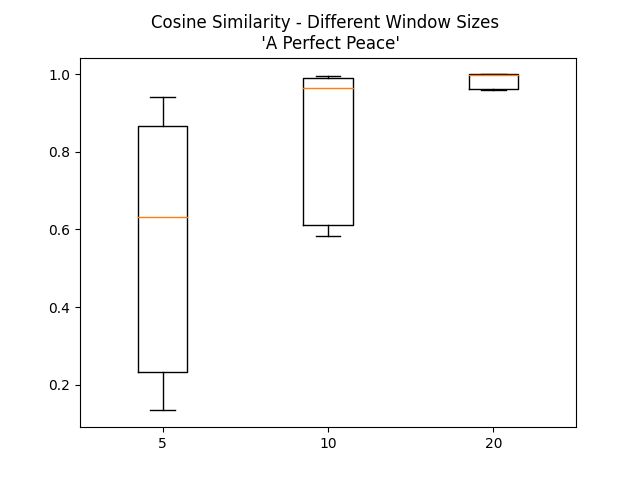
\includegraphics[width=0.75\textwidth]{Figs/window_size.png}
    \caption{Window Sizes Box Plot}
    \label{fig:win_size}
\end{figure}

\section{Single-Book Visualizations and Model Comparison}
\label{sec:single_book_visualizations}

The visualization of model outputs and their discrepancies forms the core of the evaluation, providing the \textquotedblleft teasers\textquotedblright{} for human interpretation. The following sections detail the visualizations derived from the in-depth analysis of Amos Oz's Books.

\subsection{Network Overviews: W2V vs. Co-occurrence}
\label{sec:network_overviews}

Before computing the discrepancy, we first visualize the character relationships generated by the individual computational models. Figures ~\ref{fig:coo_heatmap} and ~\ref{fig:w2v_heatmap} present the raw weighted adjacency matrices as heatmaps for two foundational networks: the Word2vec distributional similarity network and the automatic co-occurrence network.

\begin{figure}[h]
    \texttt{h}
    \centering
    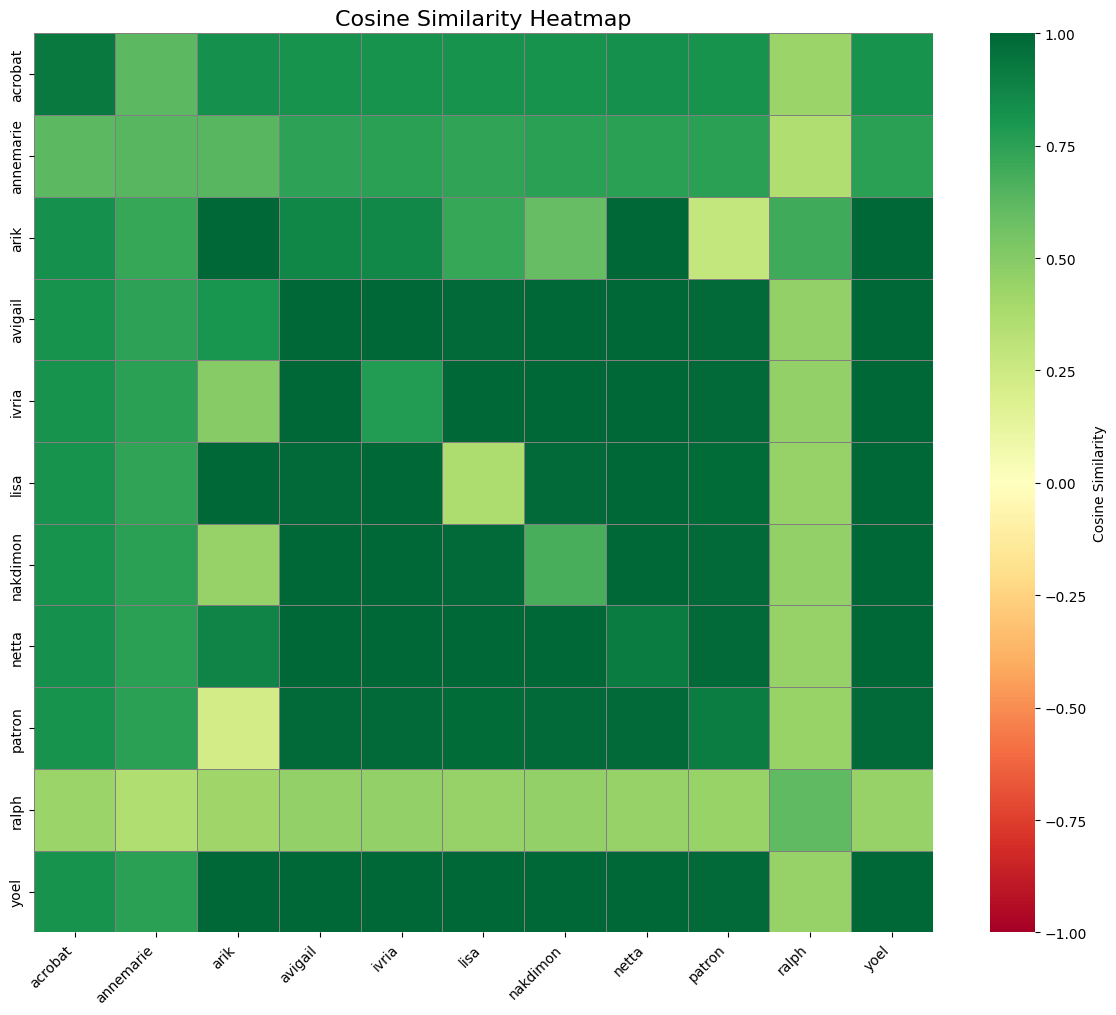
\includegraphics[width=0.7\textwidth]{Figs/W2V heatmap.png}
    \caption{The Word2vec distributional similarity network of \textquotedblleft To Know A Woman\textquotedblright{}, represented as a heatmap of the weighted adjacency matrix.}
    \label{fig:w2v_heatmap}
\end{figure}
\begin{figure}[h]
    \texttt{h}
    \centering
    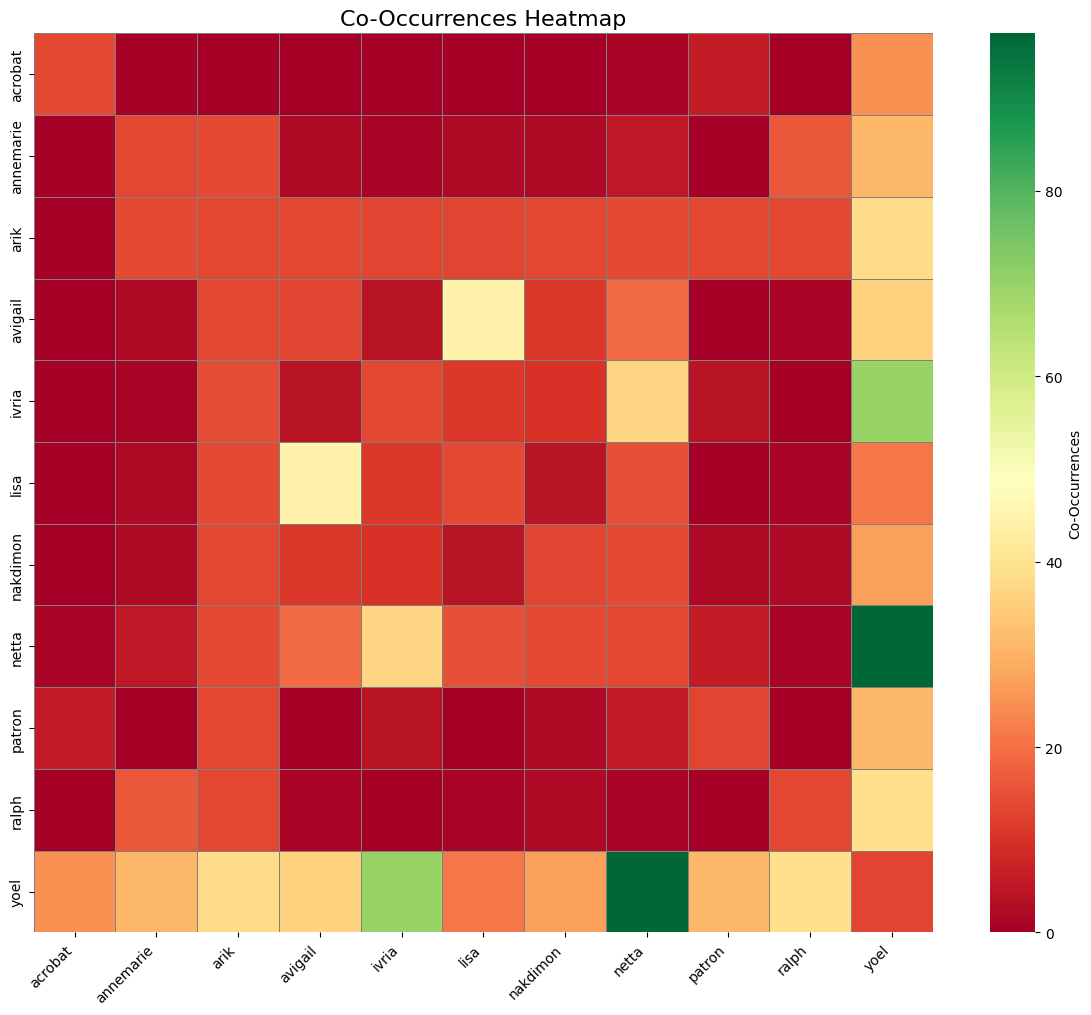
\includegraphics[width=0.7\textwidth]{Figs/CoOc heatmap.png}
    \caption{The Co-occurrences network of \textquotedblleft To Know A Woman\textquotedblright{}, represented as a heatmap of the weighted adjacency matrix. }
    \label{fig:coo_heatmap}
\end{figure}
Even at this raw stage, a qualitative comparison shows that each network tells a slightly different story. Notably, the \textbf{Word2vec} network grants centrality to minor characters (e.g., Nakdimon) through semantic relatedness, whereas the \textbf{co-occurrence} network emphasizes the core family triangle (Yoel, Netta, Ivriya) based on physical proximity. These differences justify the need for discrepancy mining.

\subsection{Computational Discrepancy Graph}
\label{sec:computational_discrepancy_graph}
\begin{figure}[h]
    \texttt{h}
    \centering
    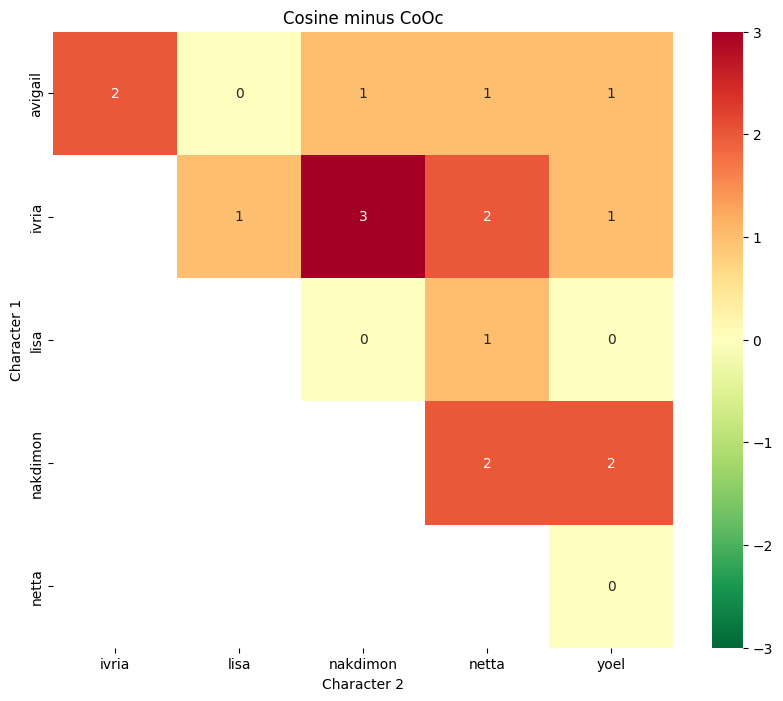
\includegraphics[width=0.8\textwidth]{Figs/Cosine minus CoOc.png}
    \caption{A Gap network visualizing the difference between the Cosine Similarity and Co-Occurrences models.}
    \label{fig:Cosine minus CoOc}
\end{figure}



The primary output of the \textbf{Clustering-Based Graph Difference (CBGD)} method is the discrepancy graph, which highlights the \textquotedblleft gaps\textquotedblright{} between the models. Figure~\ref{fig:Cosine minus CoOc} visualizes the difference between the Word2vec Cosine Similarity and the Co-occurrence networks.


The colors represent the difference in cluster assignments ($w_{ab}^{\Delta} = c_{ab}^{(W2V)} - c_{ab}^{(COO)}$): warmer color indicates higher cosine similarity (semantic bond) than co-appearance, while greener indicates the opposite (high co-appearance despite weak semantic connection).



\subsection{Comparison with Manual Network}
\label{sec:comparison_manual_network}

To evaluate the degree of divergence between automatic and human-curated relationships, we incorporate the manually created conversational network. Figures~\ref{fig:CoOc minus Manual} and \ref{fig:Cosine minus Manual} illustrate the subsequent discrepancy graphs (corresponding to Figures 7 and 8 in the paper):
\begin{enumerate}
    \item \textbf{Figure~\ref{fig:Cosine minus Manual} (Cosine vs. Manual Counting):} Compares the semantic network to the annotated conversational flow.
    \item \textbf{Figure~\ref{fig:CoOc minus Manual} (Automatic Co-occurrence vs. Manual Counting):} Compares the two count-based methods, one fully automated and the other human-curated.
\end{enumerate}

\begin{figure}[h]
    \centering
    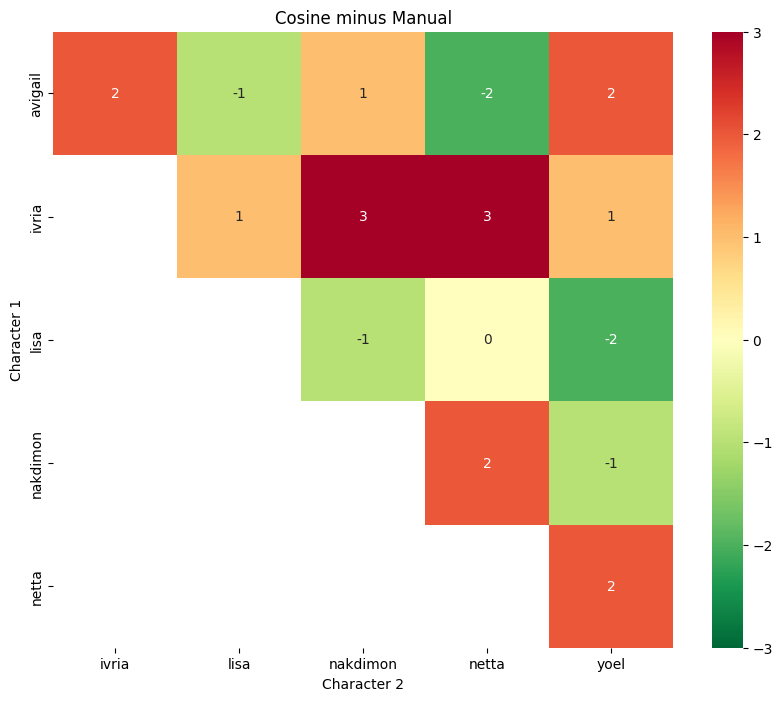
\includegraphics[width=0.8\textwidth]{Figs/Cosine minus Manual.png}
    \caption{A Gap network visualizing the difference between the Cosine Similarity and Manual Conversational Counting.}
    \label{fig:Cosine minus Manual}
\end{figure}

\begin{figure}[h]
    \centering
    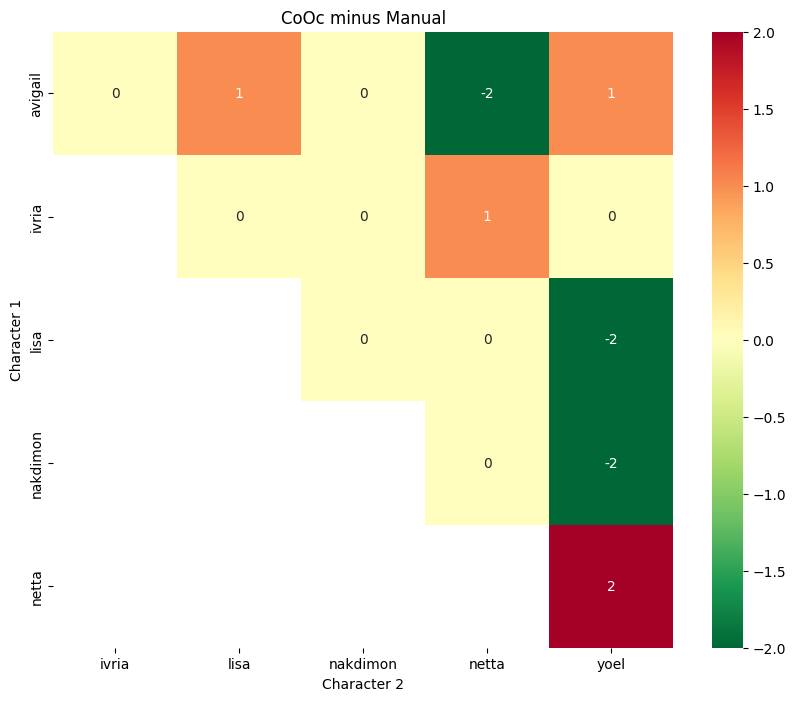
\includegraphics[width=0.8\textwidth]{Figs/CoOc minus Manual.png}
    \caption{A Gap network visualizing the difference between the Automatic Co-occurrences Counting and Manual Conversational Counting.}
    \label{fig:CoOc minus Manual}
\end{figure}
\subsection{Correlation Between Lenses}
\label{sec:correlation_between_lenses}

To quantitatively assess the structural overlap between the different character relationship models, we compute the \textbf{Spearman correlation matrix} using the raw edge weights of each lens. This normalized approach allows for a direct comparison of rankings across models with disparate scales (e.g., Co-occurrence counts vs. Cosine Similarity).

\begin{figure}[h]
    \centering
    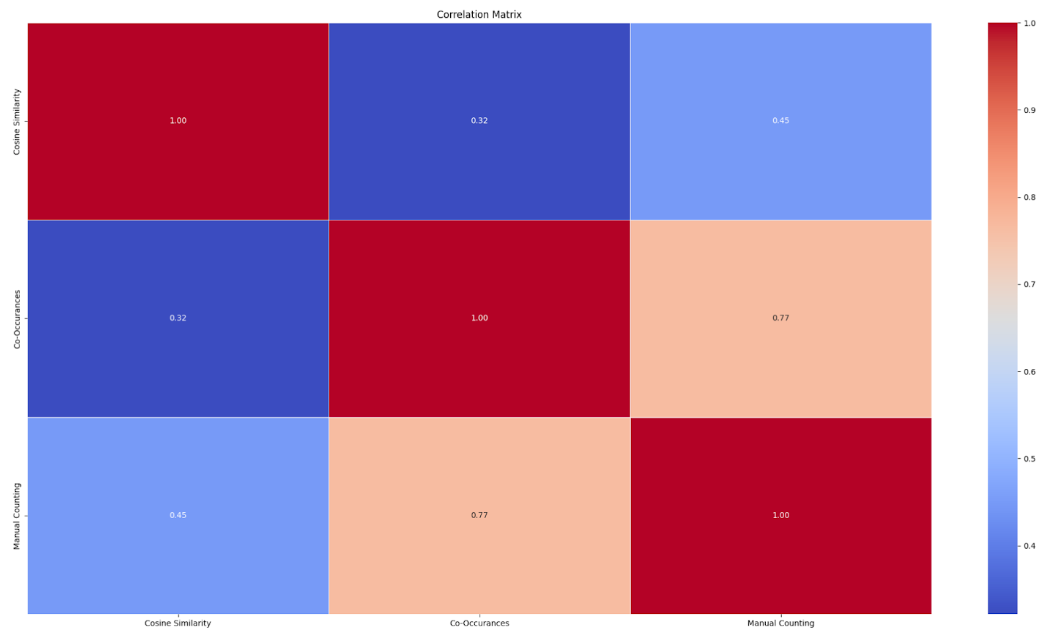
\includegraphics[width=0.75\textwidth]{Figs/correlation between lenses.png}
    \caption{Correlation Matrix}
    \label{fig:correlation}
\end{figure}

The correlation matrix, exemplified in Figure~\ref{fig:correlation} for \textquotedblleft To Know A Woman\textquotedblright{}, confirms that the models capture complementary information. The manual-based conversational and automatic co-occurrence networks show a moderate to high correlation, as expected. Critically, the cosine similarity model demonstrates a nuanced alignment, correlating more strongly with human-annotated manual counting ($\approx 0.45$) than with the automatic co-occurrence ($\approx 0.32$). This divergence justifies the discrepancy-based approach, as no single model perfectly captures the information present in the others.

\subsection{Interpretive Alignment of Computational Results}
\label{sec:correlation_between_lenses}
Taken together, the visualizations, discrepancy graphs, and correlation analyses demonstrate that the computational models do not merely generate alternative network structures, but capture distinct and narratively meaningful dimensions of character relations.

In \textit{To Know A Woman}, the low-discrepancy core triangle (Yoel–Netta–Ivria) reflects both high co-occurrence and high semantic similarity. This computational convergence aligns with traditional literary interpretation, which positions these characters as the emotional and structural center of the novel. The agreement between lenses therefore reinforces established close-reading insights.

More revealing are the high-discrepancy “hot spots.” Characters such as Nakdimon, who appear relatively infrequently yet show strong embedding-based similarity to the protagonists, occupy a marginal position in proximity-based networks but a central one in semantic space. This divergence suggests latent thematic or psychological resonance. Rather than being incidental figures, such characters may embody suppressed tensions, ideological contrasts, or symbolic reflections of the protagonists.

Conversely, pairs that frequently co-occur yet exhibit weak semantic similarity—such as Lisa and Avigial—highlight relationships grounded in spatial or situational proximity rather than deep thematic alignment. The discrepancy thus differentiates between types of relational bonds: physical, dialogical, psychological, and symbolic.

These observations support the central claim of this thesis: computational discrepancies are not arbitrary artifacts of modeling variation, but structurally informative signals. The gap network functions as a heuristic device that directs interpretive attention toward zones of representational tension. In doing so, it operationalizes the broader theoretical premise introduced in Chapter~\ref{sec:intro}: that divergence between computational lenses can serve as a productive trigger for renewed literary analysis.

\section{Cross-Book Analysis}
\label{sec:cross_book_analysis}

The discrepancy framework is extended to facilitate \textbf{cross-book analysis}, allowing researchers to investigate thematic connections and character archetypes across multiple novels by Amos Oz.

\subsection{PCA of Character Embeddings}
\label{sec:pca_embeddings}

To visualize the overarching relationships between characters from different novels, we project the 200-dimensional Word2vec character embeddings from five different novels into a 2D space using \textbf{Principal Component Analysis (PCA)}. This visualization (Figure~\ref{fig:pca}, allows for the identification of semantic clusters that bridge different literary works.

\begin{figure}[h]
    \centering
    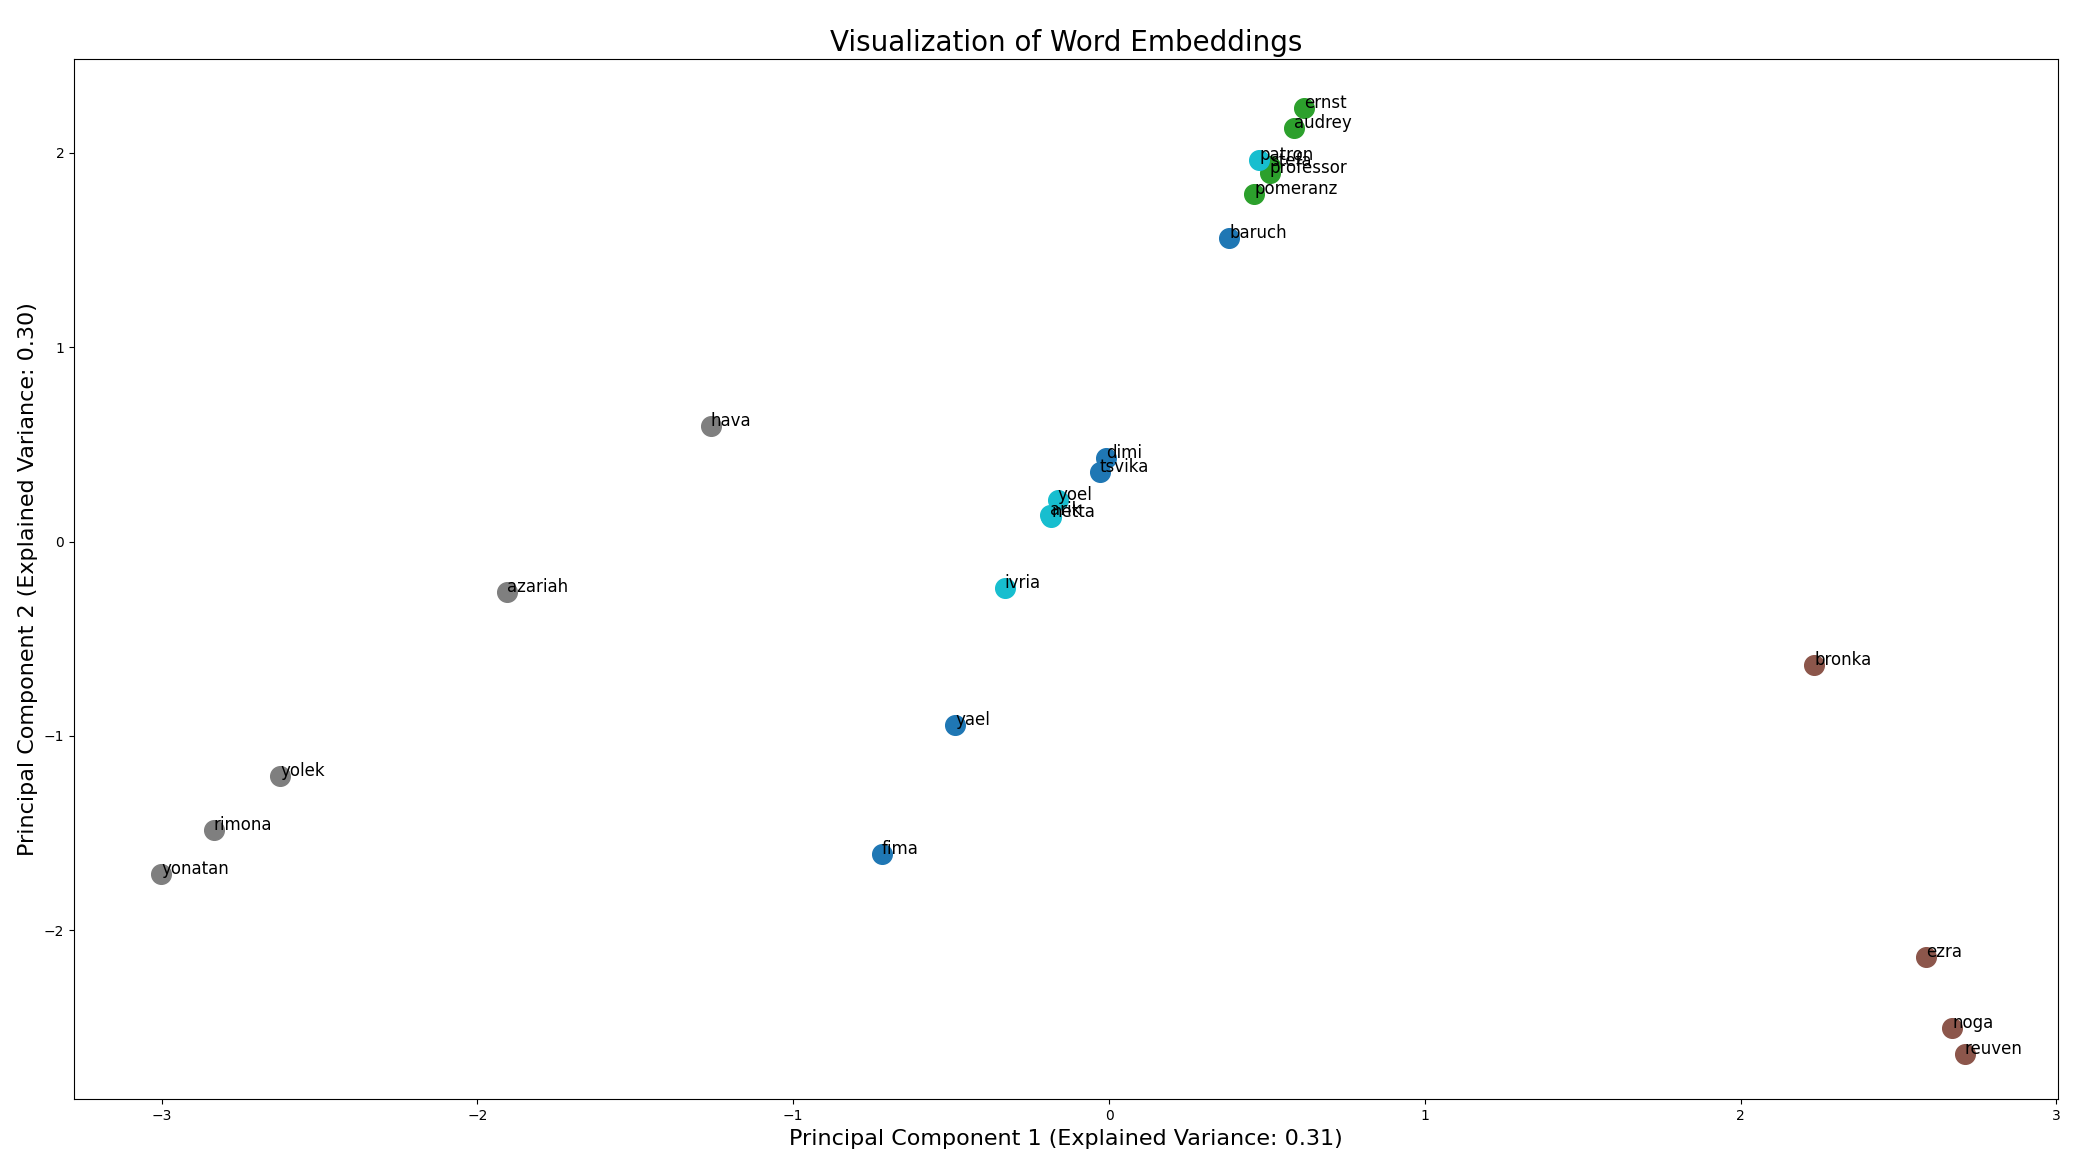
\includegraphics[width=0.8\textwidth]{Figs/pca.png}
    \caption{PCA Projection of Character Embeddings to a 2D Space. Characters from the same book are given the same color, illustrating natural within-book clustering and inter-book semantic links.}
    \label{fig:pca}
\end{figure}

The visualization shows that character embeddings from the same book tend to project onto an \textbf{almost similar vector direction} in the 2D space, reflecting the contextual and semantic similarity inherent to characters within a single narrative unit. However, the visualization's primary value lies in showing when a character from one novel may be more semantically related to a character from another, serving as a powerful teaser for cross-book reading.



%%%%%%%%%%%%%%%%%%%%%%%%%%%%%%%%%%%%%%%%%%%%%%%%%%%%%%%%%%%%%%%%%%%%%%%%%%%%%%%%%%%%%%%%%%%%%%%%%%%
%%%%%%%%%%%%%%%%%%%%%%%%%%%%%%%%%%%%%%%%%%%%%%%%%%%%%%%%%%%%%%%%%%%%%%%%%%%%%%%%%%%%%%%%%%%%%%%%%%%
\newpage
\chapter{Future Work: Qualitative Validation}
\label{chap:future_work}

The primary directive for future work is the culmination of the research methodology: the execution and analysis of the \textbf{Phase II Qualitative Evaluation} (\ref{sec:reader_oriented_evaluation}). This involves finalizing the structured $\text{Qualtrics}$ survey instrument, distributing it to the collaborating literary scholars, and rigorously analyzing the resulting empirical data. The ultimate goal is to move beyond the computational output by \textbf{quantitatively confirming the core hypothesis}: that the calculated network $\text{discrepancies}$ ($\text{gaps}$) function as powerful, non-trivial interpretive $\text{teasers}$ that meaningfully enrich the human close reading process.
%%%%%%%%%%%%%%%%%%%%%%%%%%%%%%%%%%%%%%%%%%%%%%%%%%%%%%%%%%%%%%%%%%%%%%%%%%%%%%%%%%%%%%%%%%%%%%%%%%%
%%%%%%%%%%%%%%%%%%%%%%%%%%%%%%%%%%%%%%%%%%%%%%%%%%%%%%%%%%%%%%%%%%%%%%%%%%%%%%%%%%%%%%%%%%%%%%%%%%%
\chapter{Conclusion}
\label{chap:conclusion}

This thesis introduced a novel, discrepancy-based framework for computational literary studies, designed specifically to capture the multidimensional complexity of character relationships often missed by conventional single-model network analysis. The core contribution is the \textbf{Clustering-Based Graph Difference ($\text{CBGD}$) method} (\ref{CBGS}), which successfully synthesizes insights from heterogeneous computational models ($\text{Co-Occurrence}$, $\text{Word2Vec}$, $\text{BERT}$) to quantify meaningful structural divergences. Experiments conducted on $\text{Amos}$ $\text{Oz}$'s novels demonstrated that these discrepancies function as powerful "teasers" (\ref{chap:experiments}), revealing hidden psychological and thematic connections—such as unexpected semantic ties between main and minor characters (\ref{sec:single_book_visualizations}) and cross-book character (\ref{sec:cross_book_analysis}) that defy obvious pattern recognition. Ultimately, this work redefines the computational product not as an end result, but as the \textbf{starting point for human heuristics}, successfully maintaining a critical and productive tension between distant and close reading. Future validation efforts will focus on empirically confirming the interpretive utility of this approach through structured qualitative surveys (\ref{chap:future_work}).

\newpage
\chapter{Bibliography}
\printbibliography
\label{bib}
\selectlanguage{english}

    \begin{titlepage}
	\begin{center}		
            
\includegraphics[width=1\textwidth]{Figs/BGU.png}\\
                \selectlanguage{hebrew}
            \huge{\textbf{שימו לב להפרשים - ניתוח חישובי מבוסס־פערים של רשתות דמויות ספרותיות}
            
            \large{מוגש לשם קבלת תואר "מגיסטר" בפקולטה להנדסה}
                        
            \Large{עומרי רפאלי\\
                       בהנחיית:  ד"ר  דן וילנצ'יק ופרופ' איתי מרינברג-מיליקובסקי}
    
                \small{ 
                    \raggedright{כותב: עומרי רפאלי}
                    \hspace{5cm}
                    \raggedright{……………}                    
                    \hspace{1.5cm}
                    \raggedright{תאריך: ………………}
                    \\
                    \raggedright{מנחה: ד"ר  דן וילנצ'יק }
                    \hspace{4.2 cm}
                    \raggedright{……………}                    
                    \hspace{1 cm}
                    \raggedright{תאריך: ………………}
            
                    \raggedright{מנחה: פרופ' איתי מרינברג-מיליקובסקי}
                    \hspace{1.4 cm}
                    \raggedright{……………}                    
                    \hspace{1 cm}
                    \raggedright{תאריך: ………………}
                    \\                    
                    \hspace{1.5cm}
                    \\
                    \raggedright{אישור יו"ר ועדת תואר שני מחלקתית:}
                    \hspace{0.05cm}
                    \raggedright{……………}                    
                    \hspace{1.5cm}
                    \raggedright{תאריך: ………………}
                    \\
                }
	\end{center}
    \end{titlepage}
 
    \begin{titlepage}
	\begin{center}			
            
\includegraphics[width=1\textwidth]{Figs/BGU.png}\\
            \selectlanguage{hebrew}
    
            \huge{\textbf{שימו לב להפרשים - ניתוח חישובי מבוסס־פערים של רשתות דמויות ספרותיות}}
    
            \vspace{1cm}
            \large{מוגש לשם קבלת תואר "מגיסטר" בפקולטה להנדסה}
            
            \vspace{1cm}
                
            \Large{עומרי רפאלי\\
                        בהנחיית: ד"ר  דן וילנצ'יק ופרופ' איתי מרינברג - מיליקובסקי}
	\end{center}
    \end{titlepage}
    
\thispagestyle{empty}
\end{document}